\documentclass[submit,techrep,noauthor]{ipsj}

\usepackage[dvipdfmx]{graphicx}
\usepackage{latexsym}
\usepackage{url}
\usepackage{xcolor}
\usepackage{listings}
\usepackage{amsmath,amssymb}

\newcommand{\todo}[1]{\colorbox{yellow}{{\bf TODO}:}{\color{red} {\textbf{[#1]}}}}
\newcommand{\ihara}[1]{\colorbox{green}{{\bf IHARA}:}{\color{blue} {\textbf{[#1]}}}}

\def\Underline{\setbox0\hbox\bgroup\let\\\endUnderline}
\def\endUnderline{\vphantom{y}\egroup\smash{\underline{\box0}}\\}
\def\|{\verb|}
%

%\setcounter{巻数}{59}%vol59=2018
%\setcounter{号数}{10}
%\setcounter{page}{1}


\begin{document}


\title{大規模言語モデルによるコード生成のための反復的な要件統合と最適化プロセス\\}

\affiliate{IPSJ}{情報処理学会\\
IPSJ, Chiyoda, Tokyo 101--0062, Japan}


\paffiliate{JU}{情報処理大学\\
Johoshori Uniersity}

\author{豊嶋 浩基}{Toyoshima Hiroki}{IPSJ}[s276157@wakayama-u.ac.jp]
\author{伊原 彰紀}{Ihara Akinori}{IPSJ}[ihara@wakayama-u.ac.jp]
\author{田井 聖凪}{Tai Sena}{IPSJ}[s2310137@wakayama-u.ac.jp]

\begin{abstract}
大規模言語モデル(LLM)はソフトウェア開発の効率化に大きく貢献するが,複雑な要件への対応は依然として重要な課題である.我々はこれまで自然言語からコードを自動生成するマルチエージェント型フレームワークであるChatDevに対して,few-shotを用いた要件の細分化と段階的開発を実施した.これにより,入出力テストに基づいた性能の向上が確認できた一方で,局所的な最適化に留まり,システム全体の品質に課題を残す.
そのため本研究では,分割された要件の統合と反復的改善の概念を組み合わせた新たな開発プロセスを提案する.具体的には,分割・生成されたコード群を対象に,全体の整合性を評価し,再統合と洗練を行うイテレーションを導入する.この反復的な最適化プロセスは,複雑なソフトウェア要件に対するコード生成品質を一段階引き上げるための,新たな開発指針となることを目指す.

\end{abstract}


\maketitle

%1
\section{はじめに}
昨今の大規模言語モデル(LLM)の急速な発達に伴い,LLMはこれまで人間が時間や労力などのコストをかけて行なっていたタスクを自動・効率化する可能性を持つことから,幅広い分野において関心を集めている.ソフトウェア紅白においても同様で,コードレビューや保安,リファクタリング,テストケース生成など,様々な場面において飛躍的に生産性を向上させうる可能性が示唆されている.その中でも,開発者の意図や要件をプロンプトとして提示し,プログラムコードを自動生成する「コード自動生成」への期待は大きいものとなっている.

一方で,複数の要求を内包し,それぞれが相互に依存し合うような「複雑・大規模な要件」を満たすコードを生成する場合,現行のLLMは脆弱である.タスク全体の難易度が向上すると,LLMが十分に推論を実施せずに,短絡的な結論を導出してしまうといった挙動も報告されており,生成されるコードの仕様の一部が欠損してしまうような使用漏れや,要件の文脈の不理解に起因するロジックの誤り,関数呼び出しやデータ型・構造などのインタフェースの不一致による整合性の破綻などが発生してしまう,といったような課題が発生してしまう.

LLMの理解や推論を補助するプロンプト技術として,思考の家庭を明示的に説明するChain of thought(CoT)や,要求を満たす例を少数提示するfew-shot学習が用いられてきた.しかし,これらは局所的な推論の補完や思考パターンをLLMに確立させるタスクには有効であるが,記述方法や実装方法などにより,同様の要件に対して多種多様な解が存在するプログラミング言語においては有効打になり得ない.

本論文では,このような課題に対して複雑な要件の細分化を実施し,細分化した要件ごとの開発における全体整合を実施し,その後生成されたとコードと細分化した要件をベースとした,要件の統合と再分割によるコード自動生成におけるプロンプト作成の最適化プロセスを提案し,各工程下でLLMに対して全体概要を明示的に提示や,分割した要件の統合と再分割というイテレーションにより,マルチエージェント型コード自動生成の品質を向上させうる事を貢献とする.

論文構成は以下の通りである.2章で本研究で使用するフレームワークやキーアイディアのベースとなる関連研究について,3章ではそれらに基づいたアプローチを述べ,4章でそのアプローチに関する実験設定やRQを列挙し,5章でそれに対する結果を提示する.6章で考察を行い,7章で妥当性の脅威について議論した上で,8章で結論を述べる.

\todo{田井くんにkiroみたいなChatDev以外のフレームワークでも同様な効果が発生するかどうかとかを調査してもらっています.ChatDevみたいに内部構造がちゃんと見れるか,分割を事前のフェーズで実施しているか,の部分についても一緒に調査してもらいます.}


%2
\section{関連研究}
\label{sec:format}

%2.1
\subsection{ChatDev: マルチエージェントによる段階的開発フレームワーク}
本研究では,設計・実装・レビュー・テストと言ったウォーターフォールモデルに則り,各フェーズをプログラマやコードレビュア,プロダクトマネージャといった役割を与えられた2つのLLMエージェント同士が対話を行いながら開発を進めるフレームワークであるChatDev\cite{qian-etal-2024-chatdev}をベースラインとして使用する.各エージェントは,プロンプトで与えられた満たすべき要件文と,1つ前の開発工程までに作成された設計やコード,テストなどの成果物をチャットを介して次のフェーズに引き渡す.引き渡されたエージェントは,それらの情報を基に検討と合意形成を行い,次フェーズに渡す成果物を生成する.

この枠組みの利点として,各開発フェーズの担当するタスクが明確である点や,フレームワーク自体の構造の確認・書き換えが可能であるため,拡張性に優れている点が挙げられる.

一方で,各フェーズにおいて開発を担当するLLMに対して,同一の要件(プロンプト)が与えられるため,多数の機能を内包するような複雑・大規模な要件の場合,各フェーズでのタスクの粒度が大きくなり,不完全なコードが生成されやすくなってしまう.


%2.2
\subsection{要件の複雑度が一定を上回ると,急にLLMの精度が落ちる}
Shojaeeら\cite{IllusionApple}は,複雑度の制御が可能な規則が明確な数学的パズル問題を用いて,LLMの最終的な解とそこに至るまでの推論過程を調査した.その結果,難易度が上昇するにつれて正答率は緩やかに低下すると同時に,複雑度が一定の閾値を超えるまでは思考に要するトークンが増加しているのに対して,閾値を超えた場合には思考のトークン数が急激に下落し,LLMの推論精度が崩壊してしまう事が確認された.加えて,推論過程の調査により,複雑度が低い場合に正解には早く到達するが,その後も不要に探索を続けてしまう過剰思考が確認されている.

このようなLLMの挙動は,高い推論能力を要する自然言語からのコード自動生成においても同様に再現されうるものであり,本研究における「要件の細分化」と「細分化後要件の統合と再分割」は,LLMの推論の最適化プロセスの1つとして重要である.


%2.3
\subsection{TOSEM}\todo{サブタイ修正}
Jiangら\cite{tosem}は,few-shotにより人間の意図をLLMを用いて小さなサブタスクへ分割する「計画フェーズ」と,分割後要件を基に段階的に生成を実施する「実装フェーズ」を併用したコード生成手法を提案した.その結果として,分割フェーズにおいて提示する分割例の最適な数はトークン数やLLMの持つ注意資源の観点から4つから8つである事や,実装フェーズにおいては,分割した要件を実装の手順書のように扱い,一括でコードを生成させる方が,段階的に開発を実施し,コード断片が作成されるような形式よりも性能が向上する事が確認された.


%3
\section{few-shot分割と再統合に基づく段階的コード生成手法}
本論文におけるアプローチでは,2.3節の方針に基づいて,自然言語の要件文をLLMを用いて細分化を行う「計画フェーズ」と,2.1節で示したChatDevの機能を拡張し,段階的に開発を実施する「実装フェーズ」の2フェーズをベースとする.

また,2フェーズにより生成されたコードに基づいて,計画フェーズで細分化した要件の統合及び,細分化を実施する.統合により分割粒度の最適化を図り,再分割により依存関係や,要求の補正を狙いとする.具体的な分割規則や,拡張設計及び統合・再分割の指標は後続の節で説明する.


%3.1
\subsection{全体概要に基づく段階的開発}
本研究では,分割済みの要件から段階的に開発を進める各ステップにおいて,LLMには開発を担当する分割後の小要件とそれまでに開発された成果物(設計・コード・テストなど)に加えて,分割前の要件を全体概要が提示され,それを基に開発が進められる.ここでいう全体概要とは,細分化した要件を論理順に統合したものを指す.このような全体概要を開発を担当する全てのLLMに与える事により,2.3節で議論されていた開発の断片化を防ぎ,全体整合性の担保を目指す.

%3.2
\subsection{few-shotによる要件分割}
few-shotによる要件細分化の安定性を図るため,本研究では著者が要件文を手動で小要件群に分割し,その分割に基づいてLLMにコードを生成する.そのコードが用意した入出力テストを全て通過した場合に,その手動で行った分割は「正しい分割」である,と定義しする.その後に,分割前の文章と分割後の文章をペアとして,few-shotの例としてLLMへ提示する.2.3節の方針に基づき,ここで与える分割例の数は8件と固定する.その後,few-shot学習を実施したLLMに対して未分割の要件を与え,分割を実施する.この際,分割数の最大数は,分割のコストを考慮し,最大数を10個に制限する.また,分割例と共「重要な機能であればあるほど前方に配置する」という命令を与え,コア機能から開発を実施し,段階的に機能を拡張する,と言た構造とする.

これらのアプローチにより,分割パターンの多様性確保とプロンプト長の管理を両立しながら,要件に含まれる要求の境界を明確化し,局所的開発の最適化を目指す.\todo{分割例を1つ提示する}

%3.3
\subsection{スナップショット差分行数に基づく要件統合}
2.2節の指針により.要件の粒度が過度に小さい場合において,LLMの注意資源や推論能力を必要以上に消費し,その結果として意図しない要求まで実装を行なってしまう「暴走」を誘発し得る.そのため,本研究では,3.2節で行った分割の粒度を再検討し,粒度が小すぎる要件を統合する手法を取り入れる.

具体的には,生成されたコードの総行数をLoC,細分化した要件数(スナップショット数と同義)をReqNumと定義し,細分化した要件文を順に $r_1, r_2, r_3,\dots,r_{ReqNum}$とラベル付けを行う.$r_i$に対応した開発が完了した時点でのコード一式をスナップショット$S_i$として取得し,連続する2つのスナップショット対を$S_{i-1}S_i$として,その差分に含まれる追加及び修正された行数を$\Delta LoC_i$ と定義する.

差分行数が以下の式(1)を下回る場合,$r_i$は粒度の小すぎる要件である,とみなし,直前の要件$r_{i-1)}$と統合する.

で生成されたコード行数linessnapを取得し,最終的に生成されたコードの総行数をLoC,細分化した要件数をReqNumとして,(1)の式を満たす場合に,その要件を1つ前の要件に統合を実施し,統合後の要件から再度コード生成を実施し,入出力テストの通過率を基に評価を行う.

\begin{equation}
    \Delta LoC_i \leq LoC / ReqNum
\end{equation}

その後に,統合した要件群を基に再度コードを生成し,統合の可否について調査を実施する.

%3.4
\subsection{統合後の要件に基づく要件の再分割}
3.3節で得られた生成結果のうち,統合後に入出力テストを全て通過したケースにおいて,当該ケースで採用した要件群を新たな分割の例と認定し,few-shotで提示する分割例と置換する.これにより,分割粒度や分割後要件の並び順などの最適化が行われ,分割精度と実装安定性の向上が期待される.



%4
\section{評価設計}
%4.1
\subsection{データセット}
本研究では,満たすべき要件が自然言語で明確に記述され,かつ入出力サンプルにより生成されたコードの正当性を評価可能である事から,競技プログラミングサイトであるAtCdoerをデータセットとして活用した.その中でも,入出力サンプルを合計541件含む,200問の問題を取得した.難易度の低い問題では要件の分割により,タスク粒度が過度に小さくなってしまう可能性を考慮して,C問題とD問題をそれぞれ100問ずつ選定した.各問題は2〜4件程度の入出力サンプルを備えており,これを評価用テストとして活用し,生成したコードの品質評価に用いる.

満たすべき要件が自然言語で書かれた問題文や,生成されたコードを評価するための入出力セットが備わっていることから競技プログラミングサイトであるAtCoder\cite{atcoder}より541件の入出力テストをもつ200問の問題を取得した.尚,難易度の低い問題では分割の必要がないことから,難易度はC問題,D問題からそれぞれ100問ずつ取得した.

尚,〜〜〜要件の理解の一貫性や再現性を担保しやすいと考えられるため,問題などの自然言語は全て英語のものを取得した.

%4.2
\subsection{実験設定}
LLMは実行ごとに生成結果にばらつきが発生するため,AtCoderの問題200問に対して,要件の細分化とコードの生成を各問題あたり3回実施することで,再現性を確保した.評価に関しては,問題ごとに提供される入出力サンプルを入出力テストとして扱い,全体のテスト通過率をベースに評価を実施する.AtCoderの問題の特性上,入出力は標準入力・出力が想定されているため,3.1節で拡張した段階的に開発を行う各LLMに対して,アプリケーションのようなインタフェースは作成しないように命令を追加した.

本研究では要件の細分化やプログラマやコードレビュアーなどの段階的コード生成において,料金と性能を考慮し,LLMとして"GPT-4o-mini"\cite{gpt-4o-mini}を使用した.


%4.3
\subsection{RQ}
本節では,本研究の効果を後続の3つの軸を定める.

%4.3.1
\subsubsection{RQ1: 全体概要の学習とfew-shotによる要件の細分化は生成されるコードのテスト通過率に影響を及ぼすか?}
LLMに対して全体概要を学習させる事で断片化抑制と整合性担保,few-shot学習による分割で正しく与えられた要件文から要求を抽出が可能かを,テスト通過率をベースに比較比較し,評価を実施する.本RQにおいては,要件の分割を行わない従来のChatDevとの比較だけでなく,対照実験のようにfew-shotのみを行わなかった場合(zero-shotによる要件の細分化と各LLMに対する全体概要共有を実施)と,全体概要の提示のみを行わなかった場合(few-shoによる要件の細分化を実施し,全体概要の共有を実施しない)場合とで比較した.

%4.3.2
\subsubsection{RQ2: 細分化した要件の再統合は,生成されるコードの品質を劣化させないか?}
3.3節で述べた「スナップショット差分行数に基づく統合指標」により,粒度が過小な要件を正しく選定可能か,過小な要件を統合が生成されるコードのテスト通過率に影響を与えるかを調査した.これは,統合する事によりテスト通過率の劣化が発生する場合,統合後の要件は統合前の要件より劣化したとみられるため,再分割の指標として「差分行数に基づく統合指標」は正しいものかを確認する事が本RQの目的である.そのため,統合後同様に同様に200問の問題に対して3回の分割とコード生成を実施し,統合前のテスト通過率と比較し,評価を行う.


%4.3.3
\subsubsection{RQ3: 再統合した要件からの要件の再分割は生成されるコードのテスト通過率を向上させうるか?}
統合後に再分割を行うコストに見合うテスト通過率の向上が確認されるかを検証し,「テスト通過率が低下・変化がない場合には,再分割は不要である」という仮説に対して実証を行う.

具体的には,統合を実施した要件と,分割前の要件文をペアとして,3.2節で手動で作成した分割例と置換を行い,再度few-shotによる要件の分割を実施し,それに基づいてコードの生成を行う.他RQ同様,テスト通過率で評価を実施する.

再分割して,テスト通過率変わらないならやる意味ないやんって話

%5
\section{結果}

%5.1
\subsection{RQ1}
200問各3回に対するテスト通過率の結果を図\ref{ses2025}に示す.要件の分割を行わない一括生成では,テスト通過率は16.48\%,few-shotや全体概要の学習を行わなかった場合にはそれぞれ40.92\%,18.92\%となり,両方を実施した場合には67.07\%となった.そのため,few-shotと全体概要の学習の2つを組み合わせる事により,テスト通過率を向上させうる事が確認された.

\todo{具体的な数字・分布を載せる}
zero-shotの場合は,テストで失敗したケースにおいても入出力でエラーが発生したケースは少なく,入出力の取り扱いは概ね正しく実装されているものの,出力不一致などによる失敗が中心であった.これは全体概要の学習により,関数の呼び出しやデータの入出力構造などをはじめとする全体の整合性が保たれる一方で,局所的推論の部分でテスト失敗となっているケースが多く確認された.一方で,全体概要の学習を行わず,few-shotのみの場合においては,タイムアウトや関数呼び出しなど,実行時の構造的不整合に起因するエラーが相対的に多くみられた.これは,局所的な構造自体は与えられているが,全体像が欠如している事による開発の断片化により発生したものであると考えられる.

以上により,全体概要の学習は生成されるコードの整合性の分野において効力を発揮し,few-shotによる要件の細分化は,要求抽出,ひいては局所的最適化に貢献しうる事が示唆される.

SESで載せた棒グラフ4つのやつ

\begin{figure}[t]
    \centering
    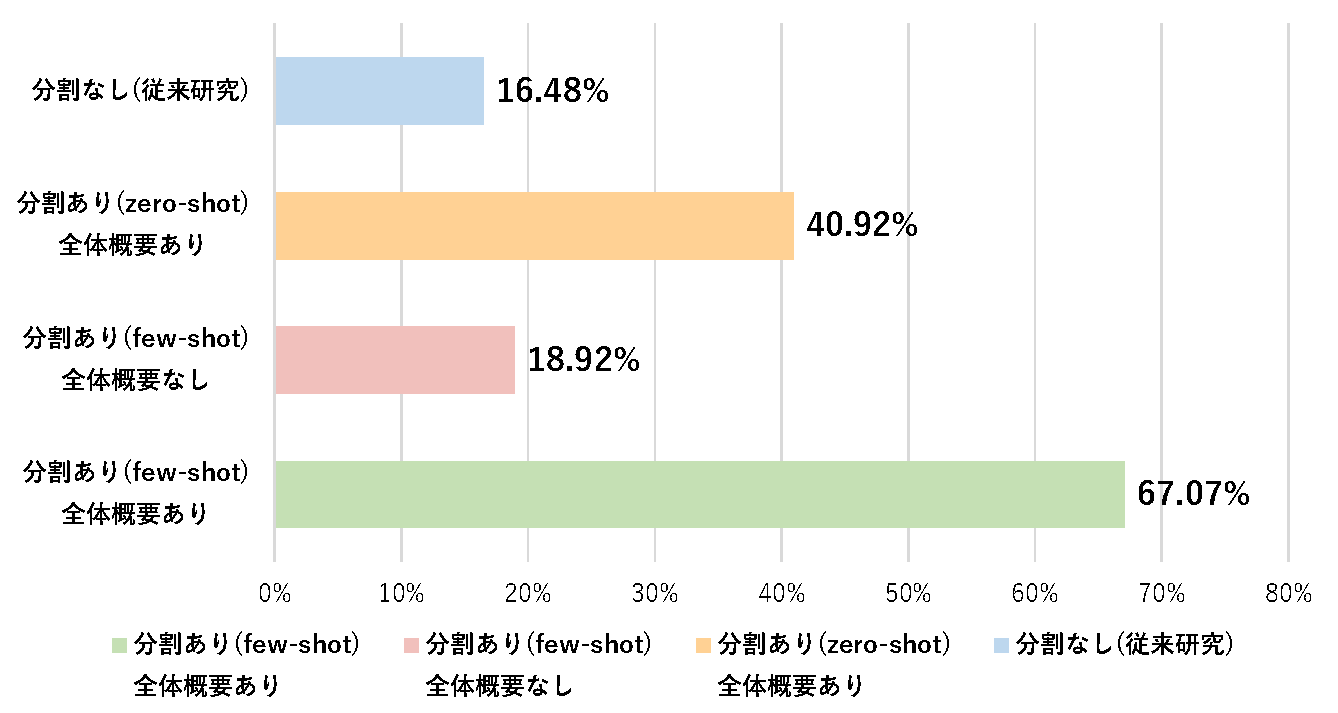
\includegraphics[width=1.0\linewidth]{./Toyoshima_fig/SIGSE_fig1.pdf}
    \caption{few-shotと全体概要の有無におけるテスト通過率比較\protect\footnotemark}
    \label{ses2025}
\end{figure}

\subsection{RQ2}
統合前
67.837\% (1,101 / 1,623)

統合後
68.762\% (1,116 / 1,623)

テスト通過率は,統合前・統合後でほぼ横ばいなので劣化は見られない.
\todo{テスト通過率だけじゃなくて,テストが通る問題の分布についても調べる(統合前なら全部通ってたのが,統合後なら通らなくなった,とかを見ていく)}

\subsection{RQ3}
統合前
67.837\% (1,101 / 1,623)

統合後
68.762\% (1,116 / 1,623)

これに対して,テスト通過率
テスト通過率(D問題100問)
85.41666\% (246 / 288)

%6
\section{考察}

%7
\section{妥当性の脅威}

%8
\section{おわりに}
\textbf{謝辞} ありがとうございました

\bibliographystyle{ipsjunsrt}
\bibliography{bibsample}

\end{document}

%memo
分割のやり直しでAI-likeな形式に変形された? イテレーション的に回していくコトでAフレンドリーな形式に変形される可能性について考察部分で持っていく